\section{Results}\label{sec:results}

\subsection{Exact optima at $n\le 22$}\label{sec:hk}
On \val{hkInstances} synthetic instances (ten each at $n=18$ and $20$, six at $n=22$; uniform and
clustered), every effort level returned the Held--Karp optimum: \val{hkHitsAll} at each of the five
levels. Held--Karp itself took \val{hk20} per instance at $n=20$ and \val{hk22} at $n=22$, against
\rt{bgma-low}{20}{ms} (\lvl{low}) to \rt{bgma-max}{20}{ms} (\lvl{max}) for BGMA (median, $n=20$). At
these sizes all levels are equivalent, and the instances are too easy to separate them. This is a
correctness check, not evidence of strength.

\subsection{Synthetic instances, $n=20$ to $400$}\label{sec:synthetic}
Table~\ref{tab:runtime} gives the median time and the mean excess over the best tour any method found,
over four instances per size (two seeds, uniform and clustered). Figure~\ref{fig:curve} plots the same
data at $n=200$ and $400$ as time against excess.

\begin{table}[t]
\centering\scriptsize
\caption{Synthetic instances: median solve time and mean relative excess over the best tour any method
found on the same instance (4 instances per cell). Excess is a \emph{relative} measure. At $n=20$ every
listed heuristic except greedy and Christofides is optimal (Section~\ref{sec:hk}).}
\label{tab:runtime}
\setlength{\tabcolsep}{3pt}
\begin{tabular}{@{}lrrrrrrrrrr@{}}
\toprule
 & \multicolumn{5}{c}{median time} & \multicolumn{5}{c}{mean excess over best found}\\
\cmidrule(lr){2-6}\cmidrule(l){7-11}
method & $n=20$ & $n=50$ & $n=100$ & $n=200$ & $n=400$ & $n=20$ & $n=50$ & $n=100$ & $n=200$ & $n=400$\\
\midrule
Greedy nearest neighbour & 3\,\textmu s & 6\,\textmu s & 13\,\textmu s & 24\,\textmu s & 50\,\textmu s & +14.03\% & +27.72\% & +31.90\% & +31.05\% & +26.46\%\\
Christofides & 220\,\textmu s & 613\,\textmu s & 1.1\,ms & 11\,ms & 27\,ms & +10.50\% & +10.07\% & +13.07\% & +13.49\% & +13.03\%\\
Beam + polish (4 restarts) & 1.1\,ms & 5.9\,ms & 43\,ms & 441\,ms & 4.10\,s & 0.00\% & +0.04\% & +0.69\% & +1.54\% & +2.22\%\\
LK-style ILS & 13\,ms & 50\,ms & 97\,ms & 672\,ms & 1.40\,s & 0.00\% & 0.00\% & 0.00\% & +0.11\% & +0.37\%\\
BGMA \lvl{low} & 1.3\,ms & 4.1\,ms & 12\,ms & 83\,ms & 622\,ms & 0.00\% & +0.12\% & +0.52\% & +1.70\% & +2.22\%\\
BGMA \lvl{mid} & 5.0\,ms & 14\,ms & 37\,ms & 222\,ms & 1.95\,s & 0.00\% & 0.00\% & +0.03\% & +0.69\% & +1.13\%\\
BGMA \lvl{high} & 9.6\,ms & 31\,ms & 84\,ms & 625\,ms & 6.37\,s & 0.00\% & 0.00\% & +0.02\% & +0.31\% & +0.60\%\\
BGMA \lvl{xhigh} & 16\,ms & 52\,ms & 212\,ms & 1.81\,s & 15.0\,s & 0.00\% & 0.00\% & 0.00\% & +0.02\% & +0.12\%\\
BGMA \lvl{max} & 65\,ms & 203\,ms & 676\,ms & 5.46\,s & 48.6\,s & 0.00\% & 0.00\% & 0.00\% & +0.01\% & +0.00\%\\
\midrule
1-tree bound (400 it.) & 96\,\textmu s & 3.5\,ms & 15\,ms & 66\,ms & 263\,ms &  &  &  &  & \\
Held--Karp & 299\,ms & --- & --- & --- & --- &  &  &  &  & \\
\bottomrule
\end{tabular}

\end{table}

\begin{figure}[t]
\centering
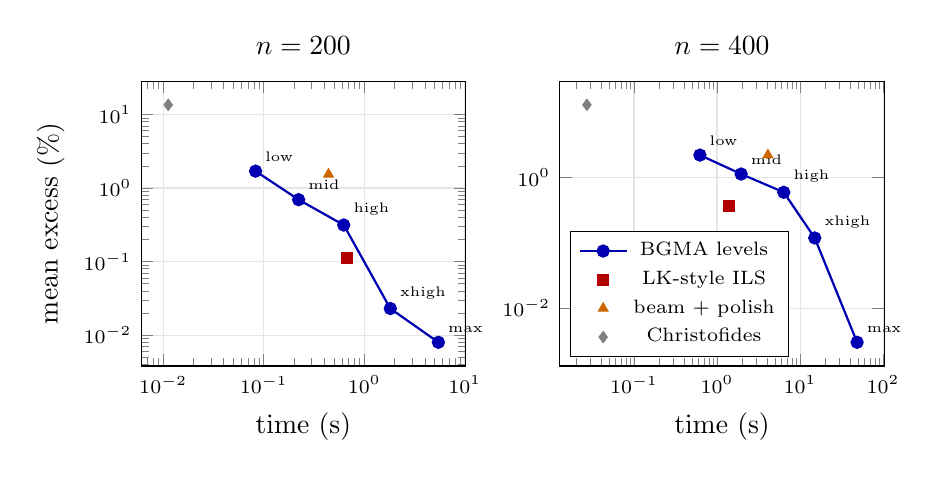
\begin{tikzpicture}
\begin{axis}[name=a0,width=0.47\textwidth,height=5.2cm,xmode=log,ymode=log,clip=false,title={$n=200$},xlabel={time (s)},ylabel={mean excess (\%)},grid=major,grid style={gray!20},legend style={font=\scriptsize,at={(0.03,0.03)},anchor=south west},tick label style={font=\scriptsize}]
\addplot[thick,mark=*,blue!70!black] coordinates {(0.08297,1.695) (0.2224,0.694) (0.6249,0.314) (1.815,0.023) (5.456,0.008)};
\node[font=\tiny,anchor=south west] at (axis cs:0.08297,1.695) {low};
\node[font=\tiny,anchor=south west] at (axis cs:0.2224,0.694) {mid};
\node[font=\tiny,anchor=south west] at (axis cs:0.6249,0.314) {high};
\node[font=\tiny,anchor=south west] at (axis cs:1.815,0.023) {xhigh};
\node[font=\tiny,anchor=south west] at (axis cs:5.456,0.008) {max};
\addplot[only marks,mark=square*,red!70!black] coordinates {(0.6718,0.111)};
\addplot[only marks,mark=triangle*,orange!80!black] coordinates {(0.4408,1.535)};
\addplot[only marks,mark=diamond*,gray] coordinates {(0.01123,13.486)};
\end{axis}
\begin{axis}[name=a1,at={(a0.east)},anchor=west,xshift=1.2cm,width=0.47\textwidth,height=5.2cm,xmode=log,ymode=log,clip=false,title={$n=400$},xlabel={time (s)},grid=major,grid style={gray!20},legend style={font=\scriptsize,at={(0.03,0.03)},anchor=south west},tick label style={font=\scriptsize}]
\addplot[thick,mark=*,blue!70!black] coordinates {(0.6224,2.215) (1.954,1.135) (6.367,0.596) (15.03,0.119) (48.63,0.003)};
\node[font=\tiny,anchor=south west] at (axis cs:0.6224,2.215) {low};
\node[font=\tiny,anchor=south west] at (axis cs:1.954,1.135) {mid};
\node[font=\tiny,anchor=south west] at (axis cs:6.367,0.596) {high};
\node[font=\tiny,anchor=south west] at (axis cs:15.03,0.119) {xhigh};
\node[font=\tiny,anchor=south west] at (axis cs:48.63,0.003) {max};
\addplot[only marks,mark=square*,red!70!black] coordinates {(1.405,0.371)};
\addplot[only marks,mark=triangle*,orange!80!black] coordinates {(4.104,2.221)};
\addplot[only marks,mark=diamond*,gray] coordinates {(0.02710,13.026)};
\legend{BGMA levels,LK-style ILS,beam + polish,Christofides}
\end{axis}
\end{tikzpicture}

\caption{Time against mean relative excess on the synthetic instances (log--log; excess floored at
0.003\% for plotting). BGMA levels are joined in order \lvl{low}$\to$\lvl{max}.}
\label{fig:curve}
\end{figure}

Five observations follow.

\emph{The dial works, at a steep price.} Each level costs about 2--3.5 times the previous one. The cost
ratios at $n=400$ are \val{ratios400}. Up to $n=400$ each level also cuts the remaining excess roughly in
half, from \rt{bgma-low}{400}{gap} at \lvl{low} to \rt{bgma-max}{400}{gap} at \lvl{max}. Fitted between
$n=20$ and $400$, time grows as about $n^{\val{expAll@bgma-low}}$ at \lvl{low} and
$n^{\val{expAll@bgma-max}}$ at \lvl{max}, but the growth steepens with $n$: between $100$ and $400$ the
exponents are \val{exp@bgma-low} and \val{exp@bgma-max}. This matches the cost model of
Section~\ref{sec:method}, in which the number of quadratic polishes itself grows with $n$. The
LK-style baseline grows as $n^{\val{exp@lkh}}$ over the same range.

\emph{From $n=200$ an LK-style ILS is the better trade-off below the top two levels.} At $n=200$ it
takes about as long as \lvl{high} (\rt{lkh}{200}{ms} against \rt{bgma-high}{200}{ms}) for about a
third of the excess (\rt{lkh}{200}{gap} against \rt{bgma-high}{200}{gap}). At $n=400$ the LK-style baseline takes
\rt{lkh}{400}{ms} for \rt{lkh}{400}{gap}. That beats \lvl{mid} (\rt{bgma-mid}{400}{ms}, \rt{bgma-mid}{400}{gap}) and \lvl{high}
(\rt{bgma-high}{400}{ms}, \rt{bgma-high}{400}{gap}) on both time and quality. \lvl{low} is faster
(\rt{bgma-low}{400}{ms}) but its excess is much larger (\rt{bgma-low}{400}{gap}). Only \lvl{xhigh} and \lvl{max} find shorter tours (\rt{bgma-xhigh}{400}{gap} and
\rt{bgma-max}{400}{gap}), and they need \val{xhighVsLk400} and \val{maxVsLk400} times the LK-style
baseline's time. At $n\le 100$ the picture reverses. Both methods are near-optimal, and BGMA's middle
levels get there faster (at $n=100$: \lvl{mid} \rt{bgma-mid}{100}{ms}, LK-style \rt{lkh}{100}{ms}).

\emph{The memetic stage earns its place over its predecessor.} The beam + polish pipeline reaches the
same quality as \lvl{low} at $n=400$ (\rt{tuned}{400}{gap} against \rt{bgma-low}{400}{gap}) but takes
\val{tunedVsLow400} times as long. Polishing every beam final is wasteful; polishing only the best
screened candidates is not.

\emph{The guarantee is far from typical behaviour.} Christofides runs in milliseconds and is
\val{chrRange} above the best found tour from $n=50$ up. From $n=50$ its
excess is \val{chrVsLow} times that of \lvl{low}.

\emph{Monotonicity across levels is not guaranteed.} Only the \lvl{max}~$\ge$~\lvl{xhigh} step is
monotone by construction (Section~\ref{sec:method}). On individual instances a cheaper level sometimes
beats a more expensive one; on rat783, for example, the \lvl{xhigh} unit beats both \lvl{max} restarts (Section~\ref{sec:tsplib}).
